\documentclass{zettel}

\renewcommand{\gregor}{\put(10.0,-3.5){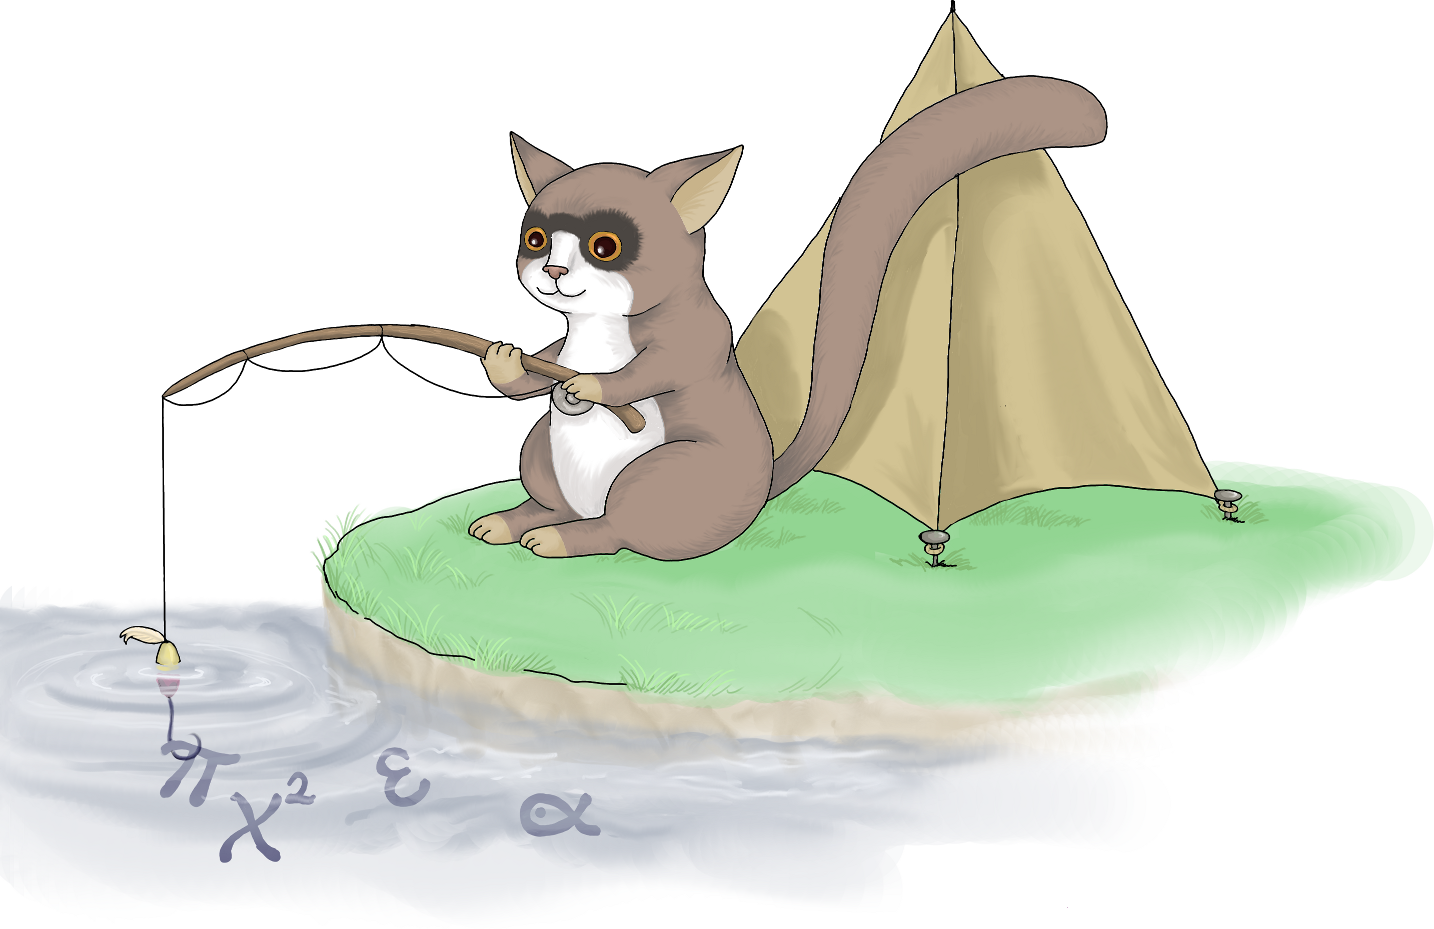
\includegraphics[scale=0.18]{campgregor}}}

\usepackage{framed}
\definecolor{shadecolor}{rgb}{.97,.97,.97}
\begin{document}

\renewcommand{\betreff}{Anmeldung zum Mathecamp des Matheschülerzirkels Augsburg}

\makeletterhead{\textsc{Bitte in Druckbuchstaben ausfüllen.}}

Hiermit melde ich meine Tochter/mein Sohn \freistLaenger{} zum Mathecamp des
Matheschülerzirkels Augsburg vom 16. bis 20. August 2014 in
Violau verbindlich an.
% (Bruder-Klaus-Heim, St. Michael Straße 15, 86450 Violau)

\vspace{-0.5em}
\doublespacing
\begin{tabbing}
  Teilnahme am: \= \kill
  Adresse: \> \freistLang \\
  \> \freistLang \\
  E-Mail: \> \freistLang \\
  Telefon: \> \freistLang \\
  Geboren am: \> \freistLang \\
  Schule: \> \freistLang \\
  Klassenstufe: \> \freistKurz
\end{tabbing}

\begin{shaded}
\textbf{Notfallkontakt.} Bei Bedarf sollen benachrichtigt werden (Name, Handy/Telefon):
\begin{enumerate}
\item \freist{7cm},\quad\freist{7cm}
\item \freist{7cm},\quad\freist{7cm}
\end{enumerate}
\end{shaded}

\begin{shaded}
\vspace{-2em}
\begin{tabbing}
  über (Vorname, Nachname): \= \kill
  \textbf{Krankenversicherung.} Mein Kind ist gesetzlich/privat krankenversichert: \\
  über (Vorname, Nachname): \> \freistLang \\
  Krankenkasse: \> \freistLang \\
  Mitgliedsnummer: \> \freistLang
\end{tabbing}
\vspace{-1em}
\end{shaded}

\newpage
\vspace*{0cm}
\singlespacing

\begin{shaded}
\textbf{Anreise.}
\begin{itemize}
\item[\checkbox] Mein Kind findet sich am 16. August zwischen 15:00 Uhr und 16:00
Uhr direkt im Bruder-Klaus-Heim in Violau ein.
\item[\checkbox] Mein Kind kommt pünktlich um 13:00 Uhr zur Universität
Augsburg und fährt dann mit einem vom Mathezirkelteam organisierten Bus nach Violau.
\end{itemize}
\end{shaded}

\begin{shaded}
\textbf{Abreise.}
\begin{itemize}
\item[\checkbox] Ich hole mein Kind am 20. August zwischen 13:00 Uhr und 14:00
Uhr direkt in Violau ab.
\item[\checkbox] Mein Kind darf direkt von Violau aus selbstständig abreisen.
\item[\checkbox] Mein Kind fährt mit dem Team zurück nach Augsburg und darf sich
ab dem Campus der Universität selbstständig auf den Heimweg machen.
\item[\checkbox] Ich hole pünktlich um 15:00 Uhr mein Kind auf dem Campus der
Universität ab.
\end{itemize}
\end{shaded}

\begin{shaded}
\textbf{Aktivitäten.}
\begin{itemize}
  \item[\checkbox] Mein Kind darf sich sportlich betätigen.
  \item[\checkbox] Mein Kind darf schwimmen.
  \item[\checkbox] Mein Kind darf in kleinen Gruppen auch ohne unmittelbare
  Aufsicht sein.
\end{itemize}
\end{shaded}

\begin{shaded}
\textbf{Sonstiges.}
\begin{itemize}
  \item[\checkbox] Mein Kind nimmt folgende Medikamente: \\[1em] \freistLang
  \item[\checkbox] Mein Kind hat folgende gesundheitliche Beeinträchtigungen
  (etwa Allergien): \\[1em] \freistLang
  \item[\checkbox] Mein Kind ernährt sich vegetarisch.
\end{itemize}
\end{shaded}

\begin{shaded}
\textbf{Mathematik.} Mein Kind hat folgende besonderen Themenwünsche: \\[1em]
\freistLang
\end{shaded}

\vfill

\begin{tabbing}
  \freistMittel \qquad\qquad \= \kill
  \freistMittel \> \freistLaenger \\
  Ort, Datum \> Unterschrift Erziehungsberechtigte(r)
\end{tabbing}

\scriptsize
Weitere Informationen und Kontaktdaten:
\textsl{http:/\!/www.math.uni-augsburg.de/schueler/mathezirkel}

\end{document}
